\documentclass[10pt]{article}

\usepackage[margin=0.78in]{geometry}
\usepackage{fontspec}
\usepackage{amsmath,amssymb,amsthm,mathtools}
\usepackage{booktabs,array}
\usepackage{enumitem}
\usepackage{graphicx}
\usepackage{xcolor}
\usepackage{microtype}
\usepackage[colorlinks=true,linkcolor=blue!55!black,citecolor=blue!55!black,urlcolor=blue!55!black]{hyperref}

\graphicspath{{./}{./toricgt_pg_softmoe_figures/}}

\theoremstyle{definition}
\newtheorem{definition}{Definition}
\newtheorem{assumption}[definition]{Assumption}
\theoremstyle{plain}
\newtheorem{theorem}[definition]{Theorem}
\newtheorem{lemma}[definition]{Lemma}
\newtheorem{proposition}[definition]{Proposition}
\newtheorem{corollary}[definition]{Corollary}
\theoremstyle{remark}
\newtheorem{remark}[definition]{Remark}

\newcommand{\R}{\mathbb R}
\newcommand{\Z}{\mathbb Z}
\newcommand{\Q}{\mathbb Q}
\newcommand{\A}{\mathcal A}
\newcommand{\G}{\mathcal G}
\newcommand{\Eop}{\mathbb E}
\newcommand{\softmax}{\operatorname{softmax}}
\newcommand{\argmax}{\operatorname*{arg\,max}}
\newcommand{\Conv}{\operatorname{Conv}}
\newcommand{\Newt}{\operatorname{Newt}}
\newcommand{\Kc}{\widehat K}
\newcommand{\norm}[1]{\left\lVert #1\right\rVert}
\newcommand{\ip}[2]{\left\langle #1,#2\right\rangle}
\newcommand{\transpose}{^{\mathsf T}}

\title{\vspace{-1.4em}ToricGT: Compact Graph-Token Reasoning with Tropical Ring Attention, Toric Diagnostics, and Random-Order Compression}
\author{Amelie Schreiber}
\date{June 1, 2026}

\begin{document}
\maketitle

\begin{abstract}
We present ToricGT, a compact graph-to-graph Transformer family for algebraic, mathematical, morphological, and parameter-constrained language-model reasoning.  The research model tokenizes nodes and edges as a shared sequence, uses exact blockwise ring evaluation for tropical max-plus attention, adds finite noncommutative-torus phase channels, and uses permutation-equivariant Soft-MoE routing in upper graph blocks.  The paper contributes a finite theory and an implementation-facing training contract.  We prove graph-token equivariance, exactness of tropical ring attention, stability of active faces under perturbation, and simulation of bounded semiring dynamic programs.  Motivated by recent toric geometry of ReLU networks, we further interpret tropical head decisions as active faces of Newton polytopes and normal fans, giving compact diagnostics for margins, bends, and future toric auxiliary losses.  A separate OpenAI Parameter-Golf track projects byte chunks to random-order graph positions and trains a dense recurrent micro language model with tied embeddings, toric position phases, tropical-ring attention, compact noncommutative-toric memory, strict-prefix GFlowNet graph-of-thought actions, BigramHash/CaseOps byte features, SmearGate confidence, stripped multi-token auxiliary heads, score-first test-time bias adaptation, and bit-packed 6-bit row-quantized export.  Its hybrid byte-TokenGT objective keeps official BPB as a byte-level prequential log score while applying causal or noncausal graph supervision to hidden reveal trajectories.  We also describe behavior-modification protocols in which learned GraphCG concept axes, toric-tropical chambers, and finite commutative-algebra certificates constrain hidden graph-of-thought trajectories to policy corridors for helpfulness, accuracy, tone, rigor, and detail.  The result is a small, auditable model design whose reasoning behavior is inspected through equivariance errors, active faces, toric moments, artifact bytes, BPB, corridor occupancy, and GFlowNet diversity rather than scalar accuracy alone.
\end{abstract}

\section{Introduction}

Many reasoning tasks are naturally graph-to-graph transformations: proof steps depend on earlier equations, graph algorithms update node and edge states, Hebrew morphology links surface forms to roots and templates, and algebraic words reduce through local rewrite relations.  ToricGT targets this regime with three design constraints.  First, relabeling a graph should relabel node and edge outputs, not change the computation.  Second, dynamic-programming-like reasoning should be visible through max-plus active faces and margins.  Third, compactness matters: the same ideas should support a small research model and a Parameter-Golf-style byte model under a strict artifact budget.

\begin{figure}[t]
  \centering
  \includegraphics[width=\linewidth]{toricgt_architecture_and_training_diagram.png}
  \caption{ToricGT combines graph tokenization, tropical ring attention, noncommutative-torus phase channels, Soft-MoE routing, and embedding-space GFlowNet fine-tuning.}
  \label{fig:arch-condensed}
\end{figure}

The main novelty is the integration of algebraic structure with trainable graph-token Transformers.  Tropical attention implements max-plus gates and exposes provenance.  Ring evaluation changes the schedule but not the function.  Finite Weyl pairs encode projective toric phase memory.  Soft-MoE gives typed differentiable routing in the research graph model.  For Parameter Golf, the same graph-token idea is compressed into random-order autoregressive decoding: each byte position becomes a graph node scored in a content-independent random order.  Finally, toric geometry supplies a new diagnostic layer: active candidates in tropical heads form exposed faces of Newton polytopes, and changes across cell walls behave like bend or Cartier-divisor intersection measurements.

\section{Model}

A ToricGT instance is
\begin{equation}
  F(G)=D\circ \Phi_L\circ\cdots\circ\Phi_1\circ T(G),
\end{equation}
where $T$ maps a typed attributed graph to node and edge tokens, $\Phi_\ell$ is a shared token-equivariant block, and $D$ is a shared node/edge/graph decoder.  A graph is
\begin{equation}
  G=(V,E,s,t,\tau_V,\tau_E,x,e,m_V,m_E),
\end{equation}
with source and target maps for edge tokens, finite node and edge types, bounded attributes, and padding masks.

\paragraph{Tropical ring attention.}
For score matrix $S$ and values $V$, a tropical head computes
\begin{equation}
  Y_{ic}=\max_j(S_{ij}+V_{jc}),\qquad
  A_{ic}=\argmax_j(S_{ij}+V_{jc}).
\end{equation}
Partitioning keys into blocks $B_1,\ldots,B_R$ gives
\begin{equation}
  \max_j(S_{ij}+V_{jc})
  =
  \max_r\max_{j\in B_r}(S_{ij}+V_{jc}),
\end{equation}
so ring evaluation is exactly equal to full tropical attention in exact arithmetic.

\paragraph{Soft-MoE routing.}
For hidden states $X\in\R^{B\times L\times d}$, learned slot vectors $\Phi\in\R^{d\times E\times S}$, and validity mask $M$, define
\begin{align}
  A_{bies}&=g\ip{x_{bi}/\norm{x_{bi}}}{\phi_{es}/\norm{\phi_{es}}},\\
  D_{bies}&=\frac{\exp A_{bies}M_{bi}}{\sum_j\exp A_{bjes}M_{bj}+\epsilon},\\
  C_{bies}&=\frac{\exp A_{bies}}{\sum_{e',s'}\exp A_{bie's'}+\epsilon},\\
  Z_{bes}&=\sum_iD_{bies}X_{bi},\qquad
  Y_{bi}=\sum_{e,s}C_{bies}f_e(Z_{bes}).
\end{align}
We use $E\ge4$ experts by default in the graph model.  The Parameter-Golf micro-LM is dense by default because a full expert bank is usually a poor bytes-per-quality tradeoff under a 16 MB artifact cap; prefix-causal or low-rank Soft-MoE remains an ablation after the dense baseline is stable.

\section{Theory}

\begin{theorem}[Graph equivariance]
If tokenization, masks, attention projections, tropical heads, Soft-MoE routing, residuals, normalization, and decoders are shared over token rows and use only equivariant incidence/type information, then ToricGT is graph-to-graph equivariant.
\end{theorem}

\begin{proof}
Tokenization maps relabeled graphs to row-permuted token tables.  Linear projections commute with row permutations.  Softmax attention, tropical attention, and Soft-MoE dispatch/combination commute with the same row permutation because their normalizers sum over either all valid tokens or slots for a fixed token.  Row-wise residual, normalization, and decoder maps commute with permutations.  Composition preserves equivariance.
\end{proof}

\begin{lemma}[Active-face stability]
If $\norm{S-\widehat S}_\infty\le\epsilon_S$ and $\norm{V-\widehat V}_\infty\le\epsilon_V$, then tropical outputs obey
\begin{equation}
  \norm{Y-\widehat Y}_\infty\le\epsilon_S+\epsilon_V.
\end{equation}
If the top-two margin is larger than $2(\epsilon_S+\epsilon_V)$, the active key is unchanged.
\end{lemma}

\begin{proof}
Each candidate score changes by at most $\epsilon_S+\epsilon_V$, and the maximum is 1-Lipschitz in $\ell_\infty$.  The margin condition keeps the original maximizer strictly above all competitors after perturbation.
\end{proof}

\paragraph{Toric diagnostic theorem.}
Let a tropical probe be $\psi(h)=\max_r(\ip{a_r}{h}+b_r)$ with rational slopes $a_r$.  Its Newton polytope is $P=\Conv(a_1,\ldots,a_R)$.  The active set
\begin{equation}
  A(h)=\argmax_r(\ip{a_r}{h}+b_r)
\end{equation}
is the exposed face of the lifted polytope $\Conv\{(a_r,b_r)\}_r$ under the linear functional $(a,b)\mapsto\ip{a}{h}+b$.  Hence tropical active-face diagnostics are cells of a normal fan.  This imports the ReLU fan / Cartier-divisor viewpoint of Fu \cite{fu2025toricrelu} into ToricGT tropical subcomputations, complementing earlier tropical rational interpretations of ReLU networks \cite{zhang2018tropical}.

\begin{figure}[t]
  \centering
  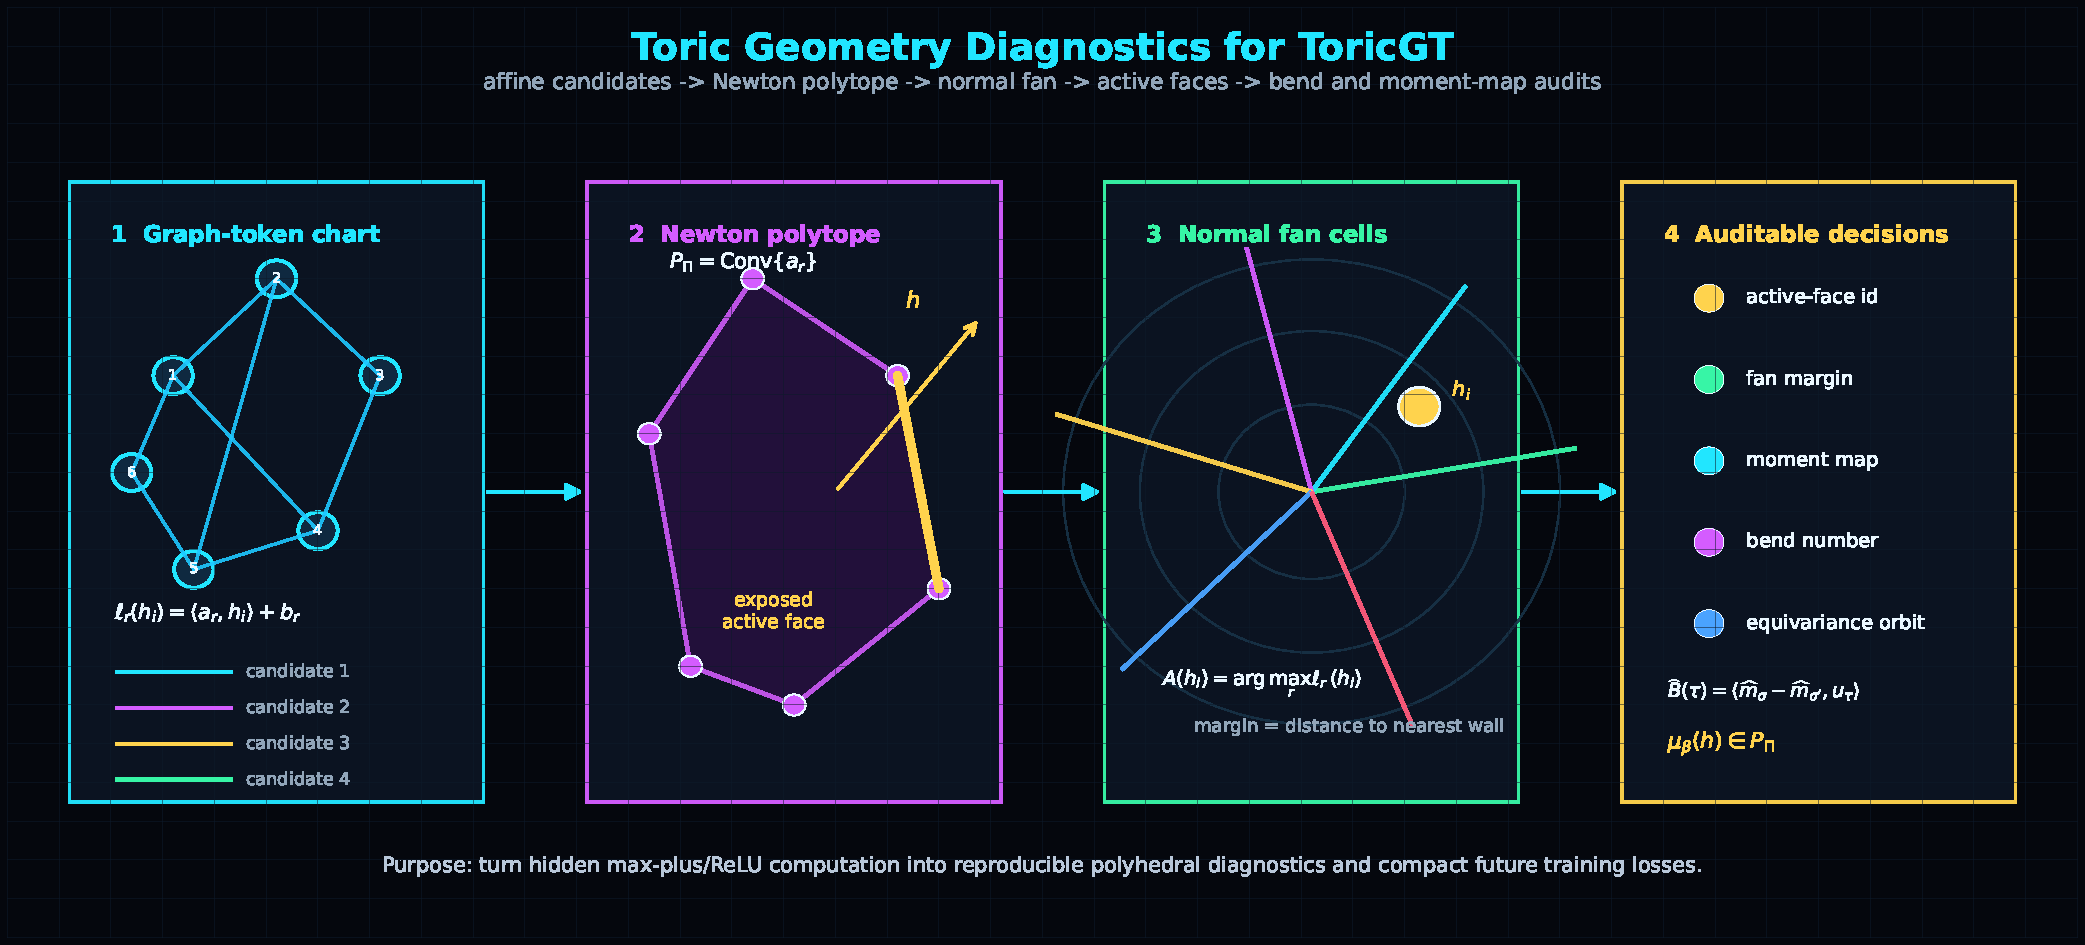
\includegraphics[width=\linewidth]{fig_toric_geometry_relu_toricgt.pdf}
  \caption{Toric diagnostics turn tropical candidate scores into Newton polytopes, normal-fan cells, active-face margins, and bend measurements.}
  \label{fig:toric-condensed}
\end{figure}

\paragraph{Finite noncommutative-toric memory.}
Let $\theta,\beta$ be rationally independent.  The competition adapter stores a small memory bank indexed by
\begin{equation}
  m_s=(\sin 2\pi s\theta,\cos 2\pi s\theta,\sin 2\pi s\beta,\cos 2\pi s\beta,
  \sin(2\pi s\theta+2\pi s\beta+2\pi s^2\theta),\cos(2\pi s(\theta-\beta))).
\end{equation}
The quadratic phase term is a finite cocycle surrogate: it gives a compact, byte-accounted way to expose clock/shift-like projective phase structure without claiming a faithful finite representation of an irrational rotation algebra.  Queries attend to these slots by cosine attention and add a small residual before logits.

\begin{proposition}[Ergodic phase coverage]
If $1,\theta,\beta$ are rationally independent, the sequence $(s\theta,s\beta)\bmod1$ is equidistributed on $\mathbb T^2$.  Consequently, finite prefixes of the toric memory supply low-discrepancy phase probes as the number of slots grows.
\end{proposition}

\begin{proof}
This is Kronecker-Weyl equidistribution.  For any nonzero $k\in\mathbb Z^2$, rational independence gives $k_1\theta+k_2\beta\notin\mathbb Z$, so the exponential averages $n^{-1}\sum_{s<n}\exp(2\pi i s(k_1\theta+k_2\beta))$ vanish.  Weyl's criterion implies equidistribution.
\end{proof}

\paragraph{Hidden-flow regularization.}
Embedding reasoning paths are treated as discrete flows $h_0,\ldots,h_T$.
Let $u_t=h_t-h_{t-1}$ and $\Delta u_t=u_t-u_{t-1}$.  The competition branch adds
\begin{align}
  \mathcal L_{\mathrm{flow}}
  &=
  \Eop_t\|\Delta u_t\|_2^2
  +\nu \Eop_t\|u_t\|_2^2 \nonumber\\
  &\quad
  +10^{-3}\operatorname{Var}_t\|h_t\|_2.
\end{align}
This is not a fluid simulation.  It is a Navier--Stokes-inspired discrete dissipation prior: high-frequency trajectory oscillations are penalized, but smooth transport through embedding space remains cheap.  The regularizer improves the stability of long GFlowNet reasoning paths and provides kinetic-energy and viscous-dissipation diagnostics for the 3D trajectory and energy-landscape plots.

\paragraph{DEC conservative reasoning flow.}
The new local-topology layer adapts a sharper idea from conservative discrete exterior calculus for incompressible Navier--Stokes on simplicial meshes \cite{mohamed2016dec}.  In DEC, incidence matrices discretize $d$, diagonal Hodge stars discretize metric duality, and conservative schemes are audited by mass, vorticity, and kinetic-energy behavior.  ToricGT uses the same algebraic pattern on reasoning complexes rather than on physical meshes.  For a reasoning window and radius $\rho$, let $A_\rho^\rightarrow$ be the directed adjacency and define the skew 1-form
\begin{equation}
  u_\rho=A_\rho^\rightarrow-(A_\rho^\rightarrow)\transpose .
\end{equation}
The DEC audit residual is
\begin{equation}
\begin{split}
  \mathcal L_{\mathrm{DEC}}={}&
  \norm{\delta u_\rho}_2^2
  +\lambda_\omega\norm{\omega_{\rho+}-\omega_\rho}_2^2
  +\lambda_E(E_{\rho+}-E_\rho)^2\\
  &+\lambda_\star\left(E_\rho^\star/E_\rho-1\right)^2
  +\lambda_\wedge\norm{u_\rho\wedge\omega_\rho-i_{u_\rho}\omega_\rho}_F^2 .
\end{split}
\end{equation}
Here $\delta$ is the row-sum divergence proxy, $\omega_\rho$ is node circulation, $E_\rho$ is edge-flow kinetic energy, $E_\rho^\star$ is the core-radius Hodge-weighted energy, and the final term is a local wedge/interior-product consistency check.  The term is small and auxiliary; its purpose is to keep long graph-of-thought trajectories conservative enough for inference-time scaling without suppressing useful directed cycle structure.

\begin{figure}[t]
  \centering
  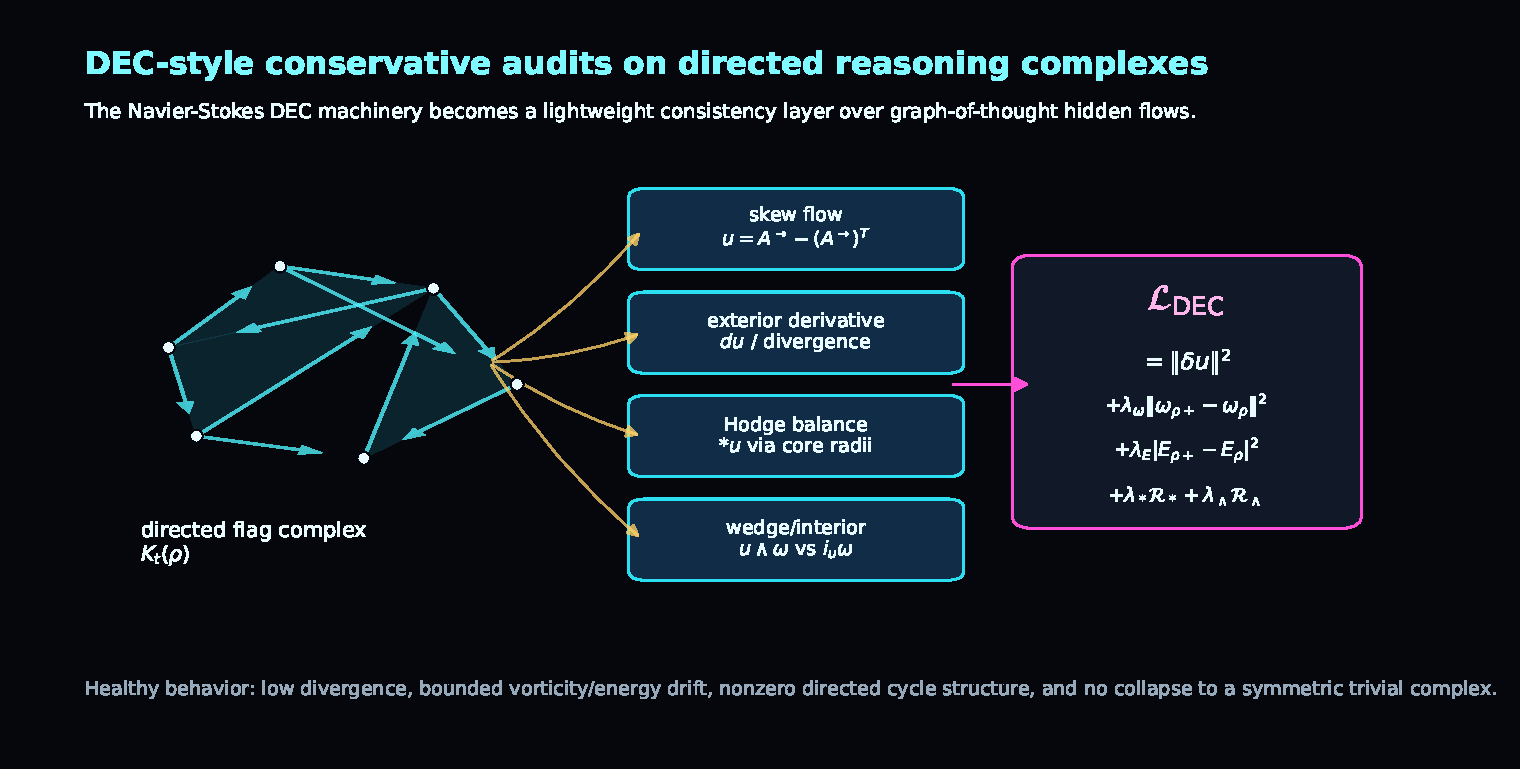
\includegraphics[width=0.98\linewidth]{fig_dec_conservative_reasoning.pdf}
  \caption{DEC-inspired conservative audits over directed reasoning complexes.  The directed graph-of-thought adjacency is treated as a discrete 1-form; divergence, vorticity drift, Hodge balance, and wedge/interior consistency become lightweight diagnostics and low-weight training signals.}
  \label{fig:dec-conservative-condensed}
\end{figure}

\section{Training And Evaluation}

The supervised objective combines node, edge, and graph losses with equivariance, torus, tropical-margin, Hebrew morphology, Soft-MoE, cache, and distillation terms:
\begin{equation}
\begin{split}
\mathcal L={}&\lambda_V\mathcal L_V+\lambda_E\mathcal L_E+\lambda_G\mathcal L_G
+\lambda_{\mathrm{eq}}\mathcal L_{\mathrm{eq}}
+\lambda_\Theta\mathcal L_\Theta+\lambda_{\mathrm{trop}}\mathcal L_{\mathrm{margin}}\\
&+\lambda_H\mathcal L_H+\lambda_{\mathrm{moe}}\mathcal L_{\mathrm{moe}}
+\lambda_{\mathrm{cache}}\mathcal L_{\mathrm{PQ}}
+\lambda_{\mathrm{KD}}\mathcal L_{\mathrm{distill}}.
\end{split}
\end{equation}
Embedding-space GFlowNet fine-tuning samples reasoning graphs with probability proportional to reward using trajectory balance.  The reward combines correctness, novelty, low equivariance error, tropical margin, low toric commutator error, and complexity penalties.

The data mixture is graph-first: math reasoning, graph-of-thought traces, algorithmic tasks, synthetic rotation/tropical tasks, Hebrew morphology graphs, and Jewish Hebrew text sources are normalized into Parquet records with stable content hashes and graph JSON.  Splits are clustered by near-duplicate text, graph sketches, algebraic normal forms, root families, and source references.

\begin{center}
\begin{tabular}{p{0.31\linewidth}p{0.53\linewidth}}
\toprule
Metric & Failure mode exposed \\
\midrule
Equivariance error & absolute-position leakage and edge-order bugs \\
Active-face margin & unstable dynamic-programming decisions \\
Toric bend consistency & incoherent polyhedral reasoning changes \\
DEC conservation residual & noisy or nonconservative hidden reasoning flow \\
Soft-MoE expert mass & expert collapse or over-routing \\
GFlowNet diversity & mode collapse and reward hacking \\
Parameter-Golf BPB/bytes & compactness and scoring compliance \\
\bottomrule
\end{tabular}
\end{center}

\section{Parameter-Golf Track}

The contest-facing model is not the full graph encoder.  It is a dense random-order byte model with tied embeddings, recurrent block reuse, toric target-position phases, lower softmax attention, upper tropical-ring attention, compact prefix-visible GFlowNet action sampling, noncommutative-toric memory slots, and byte-accounted export.  The artifact budget is
\begin{equation}
  B_{\mathrm{art}}=B_{\mathrm{code}}+B_{\mathrm{weights}}+B_{\mathrm{tokenizer}}+B_{\mathrm{metadata}}
  \le16{,}000{,}000.
\end{equation}
For a byte chunk $b=(b_1,\ldots,b_T)$, sample a content-independent order $\pi\in S_T$ from public metadata and factor
\begin{equation}
  q_\theta(b\mid \pi)=\prod_{k=1}^Tq_\theta(b_{\pi_k}\mid b_{\pi_{<k}},\pi_{\le k}).
\end{equation}
BPB is computed prequentially: predict a normalized next-byte distribution, score the observed byte, then update the state.  Because $\pi$ is independent of unscored byte values and row $k$ never contains $b_{\pi_k}$, random-order decoding is score-before-update valid while exposing more graph-like order diversity than ordinary left-to-right decoding.  A byte-safe GFlowNet policy samples latent graph-of-thought action embeddings from the prefix-visible hidden state, and validation can average multiple action samples.  Dense recurrence is the default because it adds computation without adding stored expert weights; Soft-MoE adapters are retained only as byte-accounted ablations.  Curated \texttt{graph\_json} records are projected into compact node/edge byte traces so graph structure is visible to this adapter.  Graph-of-thought trajectories are modeled as branch/merge DAGs \(G_\tau=(V_\tau,E_\tau)\), not as single lines: vertices with \(\operatorname{outdeg}>1\) explore alternatives, vertices with \(\operatorname{indeg}>1\) join or reconcile them, and the local diamond \(a\to\{b,c\}\to d\) is the basic cell.

The current hybrid keeps this byte distribution as the official scored object
and adds a TokenGT-style hidden-graph objective.  For reveal hidden states
$h_i$ at byte positions $p_i=\pi_i$, local path edges are
$A_{ij}=\mathbf 1\{0<|p_i-p_j|\le r\}$ and causal labels are
$E_{ij}=A_{ij}\mathbf 1\{i<j\}$ whenever such an orientation is meaningful.
Cyclic or noncausal sources instead use $E_{ij}=A_{ij}$ and turn off direction
and cycle penalties.  A compact version of the loss is
\[
  \mathcal L_{\rm ByteTokenGT}
  =
  a_e{\rm BCE}(\langle\bar h_i,\bar h_j\rangle/\tau,E_{ij})
  +a_p{\rm SmoothL1}(d_h(i,j),\log(1+|p_i-p_j|))
  +a_d\mathbb E_{i\to j}\max(0,m-\cos(h_j-h_i,\phi(p_j)-\phi(p_i)))^2
  +a_{\rm cyc}\mathbb E_{i>j,A_{ij}=1}\sigma(\langle\bar h_i,\bar h_j\rangle/\tau).
\]
Thus FineWeb is graph-structured as a sequential path graph for training, but
the reported Parameter-Golf metric remains byte-denominated BPB.
The current byte-accounted hybrid config uses $d=448$, $8$ heads, seven stored
dense blocks, and two recurrent passes; its 6-bit row-quantized LZMA artifact
probe is $15{,}206{,}131$ bytes, leaving $793{,}869$ bytes below the
$16{,}000{,}000$ byte cap.

The current competition branch adds several high-impact modifications inspired by OpenAI's public Parameter-Golf retrospective while excluding JEPA.  BigramHash gives a tiny strict-prefix n-gram memory; CaseOps adds byte-class operator features; SmearGate learns input-dependent confidence; stripped multi-token heads improve hidden states but are omitted from the artifact; contrastive hidden-state regularization replaces JEPA-style prediction; coprime row striding changes data order without changing data; score-first output-bias adaptation updates only after a token has been scored; and bit-packed 6-bit row quantization with LZMA reduces serialized weight cost.  Domain tags emphasize math, code, graph, Hebrew, biomedical, biochemical, biophysical, and toric records without adding evaluator dependencies.  The local mirror of \texttt{AmelieSchreiber/toricgt-curated-splits} is used in the competition-safe split: train shards feed supervised BPB optimization, validation shards feed score-first validation, and test shards are reserved for held-out GFlowNet test-time scaling.  The byte loader packs multiple source rows into one chunk; after warmup the training iterator switches to larger technical records, and a 2048-byte packed-context config can resume from a 1024-byte checkpoint by resizing only the learned position table.  This exploits the tropical-ring upper layers for longer composite reasoning trajectories while preserving the strict prequential scoring contract.

The next inference-scaling layer is anticipative trajectory memory.  Completed graph-of-thought DAGs are stored as compact keys
\begin{equation}
  k(\tau)=\operatorname{norm}\big[\bar h,\;h_{\mathrm{sink}}-h_{\mathrm{root}},\;v(\tau),\;\kappa(\tau),\;\rho_{\mathrm{VR}}(\tau),\;\phi_\theta(\tau),\;\phi_\beta(\tau),\;d_{\mathrm{DAG}}(\tau),\;q(\tau)\big],
\end{equation}
where \(v,\kappa\) summarize speed and curvature, \(\rho_{\mathrm{VR}}\) is a local simplicial density/radius statistic, \(\phi_\theta,\phi_\beta\) are noncommutative toric phase-shadow moments, \(d_{\mathrm{DAG}}\) records branch count, merge count, branch diversity, merge scatter, and back-edge fraction, and \(q\) is a trajectory-quality proxy.  A small retrieval head predicts which memory item helps the current state:
\begin{equation}
  r_\psi(s,i)=\frac{\ip{Q_\psi(s)}{K_\psi(k_i)}}{\tau_r}.
\end{equation}
During training, an in-batch teacher favors low-NLL trajectories with aligned GraphCG charts, toric phases, and local topology,
\begin{equation}
  \tilde r(s,i)=\lambda_G\ip{g_s}{g_i}+\lambda_\Theta\ip{\phi_s}{\phi_i}-\lambda_T d_{\mathrm{top}}(s,i)+\lambda_D\ip{d_{\mathrm{DAG},s}}{d_{\mathrm{DAG},i}}+q_i,
\end{equation}
and optimizes cross-entropy, KL distillation, and quality regression.  The current implementation enables this head for checkpoint compatibility but gates its loss to zero during BPB-first recovery; later GFlowNet/GraphCG/topology phases activate it at small weight.  Because retrieved helpers are completed training trajectories or legal score-before-update state, the mechanism remains compatible with prequential scoring.

\paragraph{Toric BGG certificates.}
The new Toric BGG layer uses finite shadows of hypertoric category $\mathcal O$, oriented-matroid category $\mathcal O$, multigraded BGG/Tate resolutions, and Euler-Koszul complexes as training certificates rather than as deployable modules \cite{braden2012hypertoric,brownerman2022tate,matusevich2005homological}.  A certificate is a small tuple of a standard-object poset, a sparse chain complex, internal-degree labels, optional Betti targets, and optional Gale-dual metadata.  The implemented low-rank probe reports
\begin{equation}
  \mathcal L_{\mathrm{TBGG}}=
  \lambda_{\partial^2}\|D_{k-1}D_k\|_F^2+
  \lambda_{\mathrm{std}}\mathrm{Leak}_{\mathrm{std}}+
  \lambda_{\mathrm{Kos}}\mathrm{KLR}+
  \lambda_{\mathrm{Gale}}\mathrm{GDC}+
  \lambda_{\mathrm{sig}}\mathcal L_{\mathrm{sig}},
\end{equation}
where the terms measure resolution consistency, standard-filtration leakage, Koszul-linearity residual, Gale-dual signature consistency, and BGG-signature smoothness.  These probes are excluded from the Parameter-Golf artifact with the other training-only heads.  In the corrected scratch configuration, the finite CCA, combinatorial-topology, and Koszul/BGG shadows are active from optimizer step $0$ at a deliberately tiny scale: the auxiliary channel starts at step $0$, uses a long warmup, is evaluated only on scheduled steps, and is capped to a minute fraction of the current cross-entropy loss.  Stronger promotion is still audit-gated, but metric visibility and micro-gradient pressure are not delayed behind a validation-BPB threshold.

Earlier \texttt{oai} recovery runs used BPB-only repair gates and kept heavier geometry mostly diagnostic.  The current \texttt{oai-advanced} scratch protocol changes that policy: CCA, combinatorial topology, GraphCG, Slepian/Pollak concentration, analogy, and Koszul/BGG shadows are present from step $0$ with micro weights, a $20{,}000$-step auxiliary warmup, and a CE-ratio cap.  The goal is not to let geometry overpower byte modeling; it is to make the finite algebraic/topological structure visible and gently trainable from the beginning.  Periodic analyses then decide whether to increase frequency or weight after checking OpenAI FineWeb BPB, exact finite CCA audits, Stanley--Reisner nonface mass, Koszul residuals, directed-filtration validity, and graph-of-thought trajectory quality.

\begin{figure}[t]
  \centering
  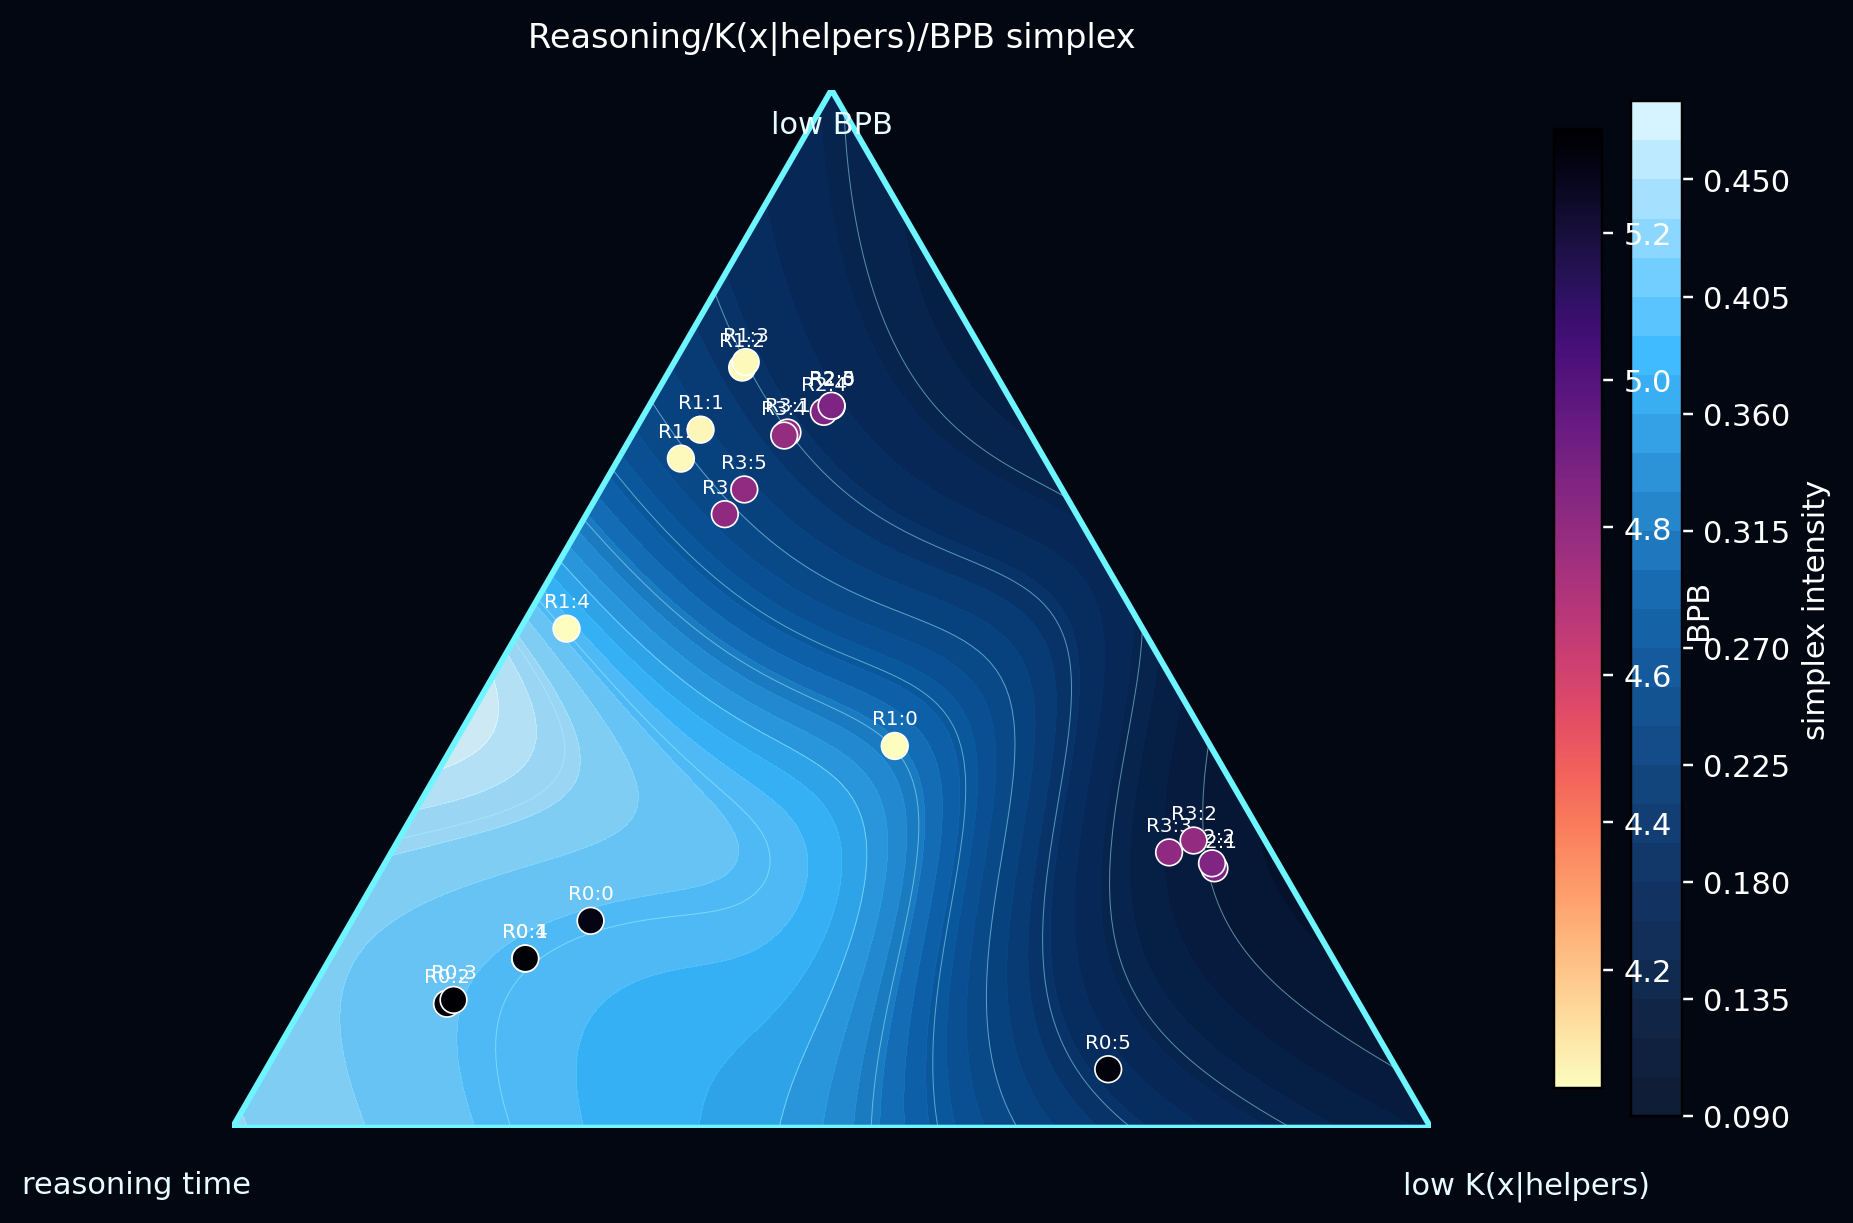
\includegraphics[width=0.86\linewidth]{fig_oai_step37250_reasoning_k_bpb.png}
  \caption{Historical step-$2250$ \texttt{oai} recovery diagnostic.  Branches are embedded in the reasoning/K$(x\mid\mathrm{helpers})$/BPB simplex from model-computed statistics.  The checkpoint still favored the low-BPB corner over longer reasoning budgets, motivating later gated GraphCG/GFlowNet promotion while heavier toric, Koszul, and Toric BGG geometry stayed gated.}
  \label{fig:oai-step2250-condensed}
\end{figure}

The \texttt{oai} branch separates two ingredients.  GraphCG learns steerable latent directions by contrasting edits along learned factors \cite{liu2024graphcg}; ToricGT uses the same idea to learn a small concept chart $B=[d_1,\ldots,d_r]$.  The analogical-reasoning paper argues that analogy emerges when relational structures align in embedding space and a functor-like map is applied by the Transformer \cite{minegishi2026analogy}.  ToricGT composes these ideas: relation arrows and graph-of-thought states are first expressed in the GraphCG chart, while analogies are modeled as filtered topological functors.  Let $h_t$ be a prefix-visible hidden state, $\xi_t=B^\top h_t$, and let $a_t=(\xi_{t+s}-\xi_t)/(\|\xi_{t+s}-\xi_t\|+\epsilon)$ be a normalized chart relation arrow.  Repeated coarse byte-relation classes are encouraged to share the same chart directions and to satisfy parallelogram closures.  For scale robustness, each relation class builds a nested soft Vietoris--Rips filtration
\begin{equation}
  A_\rho(i,j)=\sigma((\rho-\|a_i-a_j\|/\operatorname{med}\|a_p-a_q\|)/\tau),
  \qquad \rho_1<\cdots<\rho_m,
\end{equation}
and penalizes inclusion violations, chain-map commutators, and soft triangle failures.  Directionality is supplied by an antisymmetric toric form
\begin{equation}
  \Omega_{ij}=\langle a_i^{(1)},a_j^{(2)}\rangle-\langle a_i^{(2)},a_j^{(1)}\rangle,
  \qquad
  A_\rho^\rightarrow(i,j)=\sigma((\rho-d_{ij}+\gamma\Omega_{ij})/\tau),
\end{equation}
so $i\to j$ and $j\to i$ may differ.  In the hard-threshold limit these adjacencies define nested Vietoris--Rips or directed flag complexes
\begin{equation}
  K_{\rho_1}\subseteq\cdots\subseteq K_{\rho_m},
  \qquad
  H_p(K_{\rho_1})\to\cdots\to H_p(K_{\rho_m}),
\end{equation}
so the intended object is a small persistence module over hidden-state analogy arrows \cite{edelsbrunner2002topological,zomorodian2005computing,cohensteiner2007stability}.  Consecutive reasoning windows also carry soft transports $P_s$ that push source complexes to target complexes:
\begin{equation}
  \widehat A_{\rho}^{s+1}=P_s^\top A_{\rho}^{s}P_s,\qquad
  \widehat A_{\rho}^{\rightarrow,s+1}=P_s^\top A_{\rho}^{\rightarrow,s}P_s .
\end{equation}
Thus the maps are functor-like, but with additional topological structure: they should preserve filtration inclusions, approximately commute with chain and boundary maps, and induce low-residual morphisms of persistence modules.  The implementation uses differentiable persistence surrogates rather than exact barcode backpropagation.  A radius-parametrized HDBSCAN gate further computes core distances $c_i$, mutual reachability $d_{\rm mr}(i,j)=\max\{c_i,c_j,d_{ij}\}$, and persistent density affinities across the same radii.  Only high-stability neighbors receive pullback weight; outlier arrows mostly stop contributing.  The finite noncommutative toric memory supplies pseudo-periodic phase coordinates $(e^{2\pi i\theta t},e^{2\pi i\beta t})$ and a quadratic cocycle surrogate; projected to a torus, these phases make recurrence, equidistribution, and directed skew visible along reasoning trajectories.  Periodic analyses render the toric phase path, local simplicial edges, and soft analogical maps in 3D, together with directed filtration curves, HDBSCAN heatmaps, Ramachandran-style phase plots, energy landscapes, and reasoning/K/BPB simplices.  The latest interactive hidden-space diagnostics additionally draw empirical active-face chamber polytopes, fitted tropical/toric wall sheets at observed chamber crossings, and a Newton-polytope shadow from the pseudo-exponents used by the fan audit; sparse/default/dense controls adjust the local simplicial radius without recomputing the run.

GraphCG also modulates the toric geometry itself.  If a tropical probe has Newton vertices $a_r$ and active chamber
\begin{equation}
  C_r=\{h:\langle a_r-a_s,h\rangle\ge b_s-b_r\ \forall s\},
\end{equation}
then in the concept chart this chamber becomes
\begin{equation}
  C_r^B=\{\xi:\langle B^\top(a_r-a_s),\xi\rangle\ge b_s-b_r\ \forall s\}.
\end{equation}
Thus GraphCG pulls Newton normal fans and affine chamber walls into a steerable basis.  Low GraphCG covariance and high chart margins mean that toric active faces are aligned with reusable concept axes rather than smeared across arbitrary hidden directions.  This is why the current recovery enables GraphCG before enabling heavier toric losses: it first improves the coordinate chart in which fan, bend, braid, and Coxeter losses will later act.

\paragraph{Behavior corridors and assistant-axis generalization.}
The same chart makes behavior steering computable.  Anthropic's Assistant Axis is a one-dimensional contrast direction in activation space: the mean Assistant activation minus the mean activation of other personas; capping activations inside a calibrated interval reduces persona drift while mostly preserving capability \cite{lu2026assistantaxis}.  ToricGT treats this as the rank-one case of a larger toric-tropical steering atlas \cite{schreiber2026tropicalquivers}.  Let $B_\ell=[d_1,\ldots,d_r]$ be the GraphCG chart at layer or reasoning vertex $\ell$, $\xi_t=B_\ell^\top h_t$, and let $\Sigma_B$ be the pulled-back normal fan of the active tropical probes.  A behavior policy $\pi$ specifies desirable coordinates for safety, epistemic caution, tone, detail, rigor, and domain style by a chamber-indexed corridor
\begin{equation}
  K_{\pi,C}=\{\xi:\ell_j(C,\pi)\le s_j(\xi)\le u_j(C,\pi)\ \forall j,\quad
  g_a(\xi)\le 0\ \forall a\},
  \qquad C\in\Sigma_B .
\end{equation}
Affine hyperplanes $\ip{\alpha,\xi}=k$ cut each chamber into alcoves.  Good behavior is not forced to a single point; it occupies an allowed polyhedral band whose width depends on task and context.  The training and inference penalty is
\begin{equation}
  \mathcal L_{\mathrm{corr}}=
  \frac1T\sum_t \operatorname{dist}(\xi_t,K_{\pi,C(\xi_t)})^2+
  \lambda_{\mathrm{wall}}\sum_{a,t}\operatorname{softplus}(\tau g_a(\xi_t))+
  \lambda_{\mathrm{occ}}\norm{\widehat\mu_{\Sigma}-\mu_\pi^\star}_2^2 .
\end{equation}
For a single Assistant direction $v$ and interval $[\ell,u]$, $B=v/\norm{v}$ and $K=[\ell,u]$ recover activation capping:
\begin{equation}
  h\mapsto h+
  \frac{\operatorname{clip}(\ip{v}{h},[\ell,u])-\ip{v}{h}}{\norm{v}_2^2}v .
\end{equation}
The ToricGT version is richer because it can regulate many disentangled axes, use different corridors in different toric chambers, and monitor wall-crossing rates, chamber occupancy, and BPB jointly.

At a graph-of-thought vertex $q_t$, the hidden state also carries a finite reasoning complex $\Delta_t$, a Stanley--Reisner ring $k[\Delta_t]$, and a small multigraded certificate.  The behavior protocol therefore adds algebraic gates:
\begin{equation}
  \mathcal L_{\mathrm{alg\text{-}beh}}=
  \lambda_{\mathrm{SR}}\sum_{F\notin\Delta_\pi}\prod_{i\in F}x_i(\xi_t)
  +\lambda_{\mathrm{binom}}\sum_{x^u-x^v\in I_A}
     \left(\ip{u}{x(\xi_t)}-\ip{v}{x(\xi_t)}\right)^2
  +\lambda_{\mathrm{res}}\norm{\partial_{t-1}\partial_t}_F^2 .
\end{equation}
Nonface mass blocks unwanted coactivations, toric-binomial residuals preserve the intended affine chart, and differential residuals keep reasoning steps compatible with the symbolic complex.  Memory retrieval is filtered through the same corridors: retrieved trajectory nodes must be close in GraphCG coordinates, compatible in chamber label, and useful under a score-valid analogy helper.  Analogical transport $P_{s\to t}$ is rewarded when it maps a source corridor and source complex to the target corridor and target complex, so the model learns to steer not only single activations but whole directed reasoning trajectories.

\begin{figure}[t]
  \centering
  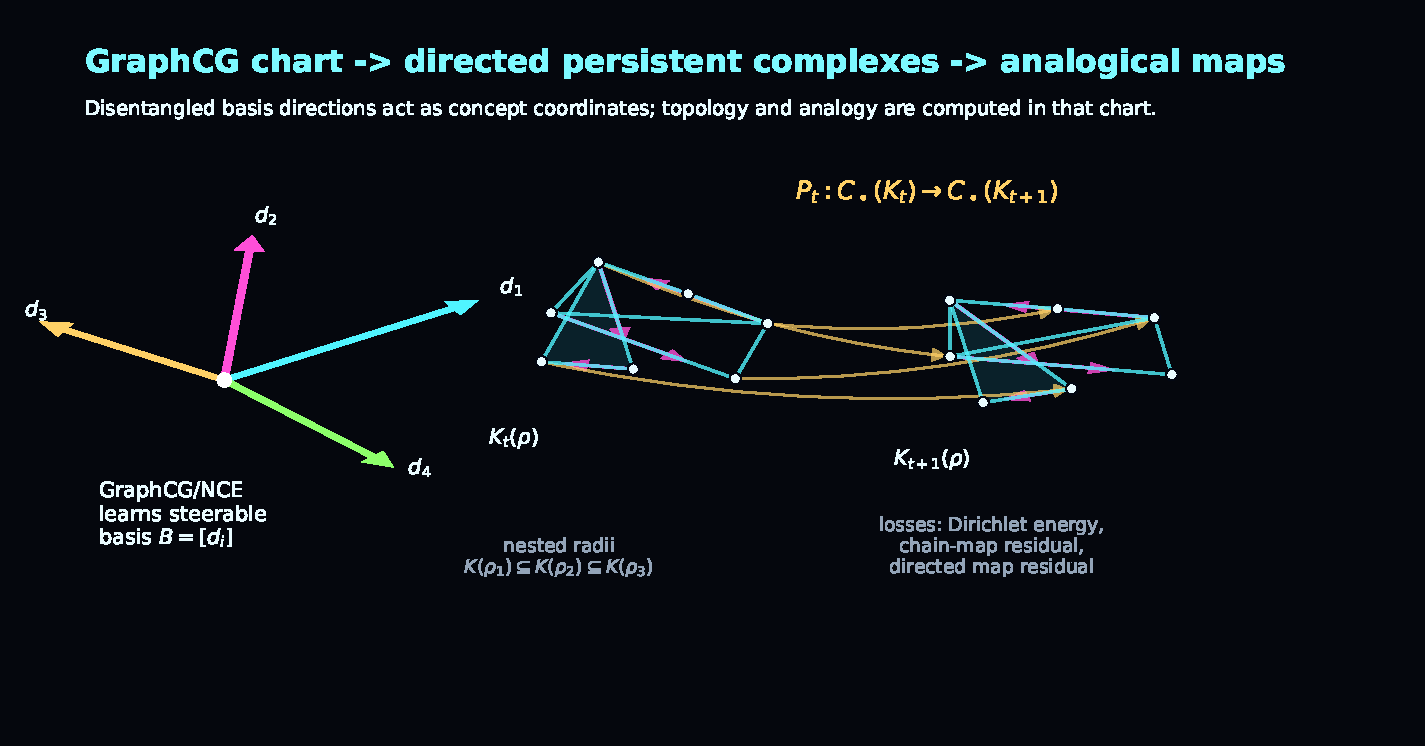
\includegraphics[width=0.98\linewidth]{fig_graphcg_topology_analogy_map.pdf}
  \caption{GraphCG supplies a steerable concept chart; ToricGT builds directed persistent complexes in that chart and learns soft functor-like maps that also preserve filtered topological structure.}
  \label{fig:graphcg-topology-condensed}
\end{figure}

\begin{figure}[t]
  \centering
  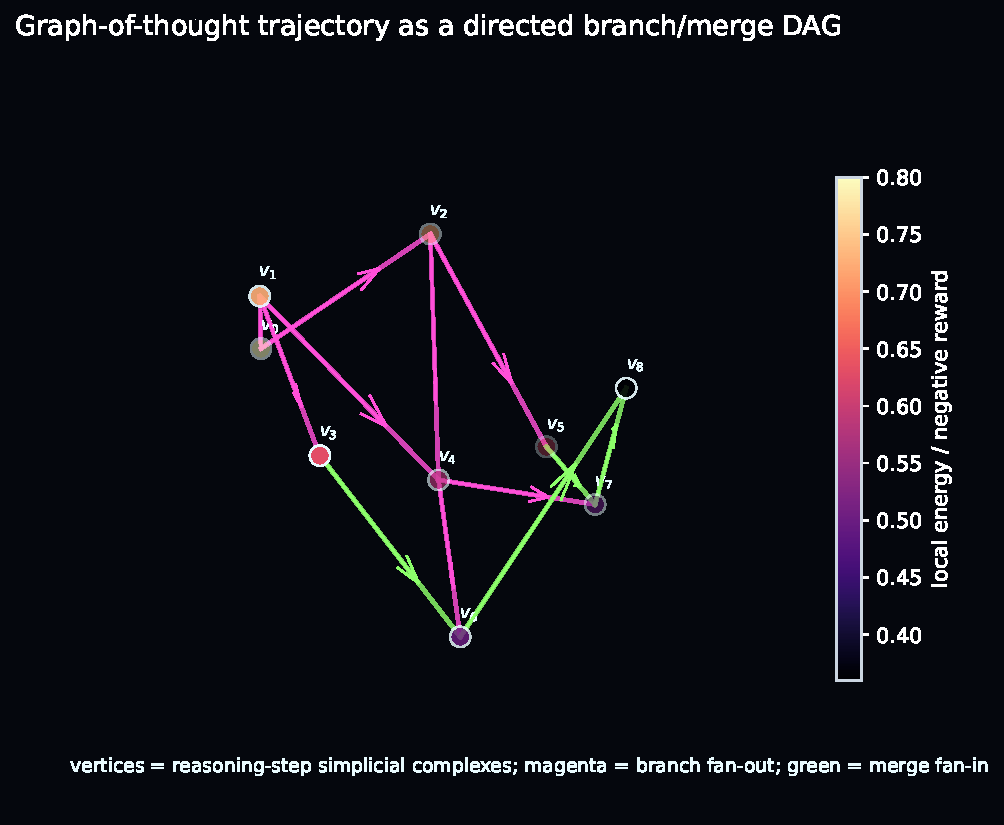
\includegraphics[width=0.86\linewidth]{fig_graph_of_thought_branch_merge_dag.pdf}
  \caption{Graph-of-thought trajectory as a branch/merge DAG.  Reasoning vertices carry local simplicial complexes and hidden-state certificates; branch fan-out explores alternatives and merge fan-in reconciles them.}
  \label{fig:got-branch-merge-condensed}
\end{figure}

\begin{figure}[t]
  \centering
  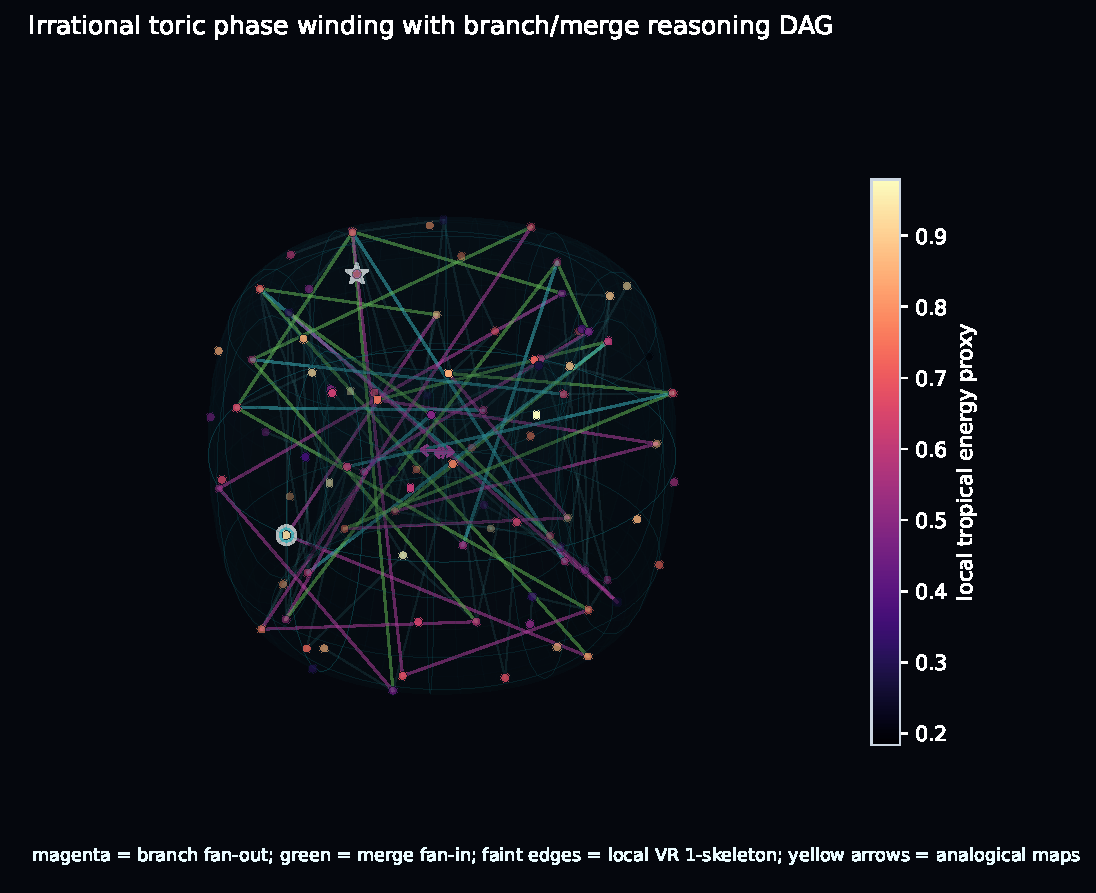
\includegraphics[width=0.86\linewidth]{fig_toric_phase_simplicial_trajectory.pdf}
  \caption{Irrational toric phase projection of a branch/merge reasoning DAG.  Vertices lie on a pseudo-periodic phase scaffold; colored directed edges distinguish branch fan-out, merge fan-in, and analogical transport.}
  \label{fig:toric-phase-simplicial-condensed}
\end{figure}

Operationally, the first serious BPB target is $1.20$--$1.22$, a strong run is $1.16$--$1.19$, an excellent run is $1.13$--$1.15$, and $\le1.12$ is exceptional under OpenAI's public recap.  Claims below $1.10$ BPB should trigger strict leakage, tokenizer, and score-before-update audits.

\paragraph{Kolmogorov-style reasoning diagnostics.}
The competition score is BPB, but BPB alone does not distinguish shallow byte compression from robust reusable reasoning.  ToricGT therefore logs estimator-tagged proxies for conditional Kolmogorov complexity.  For compressor $c$,
\begin{equation}
  \Kc_c(s)=|c(s)|,\qquad
  \Kc_c(y\mid x)=\max\{0,\Kc_c(x\,\Vert\,y)-\Kc_c(x)\},
\end{equation}
as a computable proxy for the ideal but uncomputable quantities
\begin{equation}
  K_U(y\mid x)=\min\{|p|:U(p,x)=y\},\qquad
  K_U(x\mid y)=\min\{|p|:U(p,y)=x\}.
\end{equation}
The forward direction measures how much extra program information is needed to produce the answer or next byte from the problem/prefix; the reverse direction measures how much of the problem structure is recoverable from the answer or trace.  A terse guess can have low forward proxy complexity while still losing explanatory information visible through high reverse conditional complexity.  ToricGT also logs a signed relative proxy
\begin{equation}
  \widetilde K_c(y\mid x;h_0)=\Kc_c(h_0\,\Vert\,y)-\Kc_c(h_0)-\Kc_c(y\mid x),
\end{equation}
where $h_0$ is a named baseline helper.  Negative values are relative compression gains over the baseline; they are not negative true Kolmogorov complexity.  For two trajectories
\begin{equation}
  \operatorname{NCD}_c(a,b)=
  \frac{\Kc_c(a\,\Vert\,b)-\min(\Kc_c(a),\Kc_c(b))}
       {\max(\Kc_c(a),\Kc_c(b))}.
\end{equation}
These are not claims to compute true Kolmogorov complexity.  They are auditable lower-tech probes for whether successful graph-of-thought paths are compact conditional programs, whether random orders induce stable programs, and whether GFlowNet terminal diversity is genuine rather than cosmetic.  The implementation logs conditional target complexity, order-program complexity, prediction-target NCD, graph-MDL summaries, and GFlowNet action-trace complexity to W\&B.  All such metrics are diagnostic by default; the BPB objective remains unchanged unless a future ablation explicitly gives a complexity reward nonzero weight.

The random-order model uses a structured helper set rather than a single string.  At step $k$, let
\begin{equation}
  H_k=\{b_{\pi_{<k}},\pi,\operatorname{chunk}(b),a_{<k},G_k,T_k\},
\end{equation}
where $b_{\pi_{<k}}$ is the strict prefix, $\pi$ is the public random-order tree program, $\operatorname{chunk}(b)$ is the graph-projected byte chunk, $a_{<k}$ are prefix-visible GFlowNet actions, and $G_k,T_k$ are optional serialized graph or tree helpers.  The implemented proxy is
\begin{equation}
  \widehat K_c(y_k\mid H_k)=\min_{h\in H_k\cup\{\varnothing\}}\widehat K_c(y_k\mid h).
\end{equation}
Analogical transfer is measured by adding a source source-target helper pair:
\begin{equation}
  \Delta K_c^{\mathrm{ana}}=
  \widehat K_c(y_t\mid H_t,x_s,y_s,G_s,T_s)
  -\widehat K_c(y_t\mid H_t).
\end{equation}
Negative $\Delta K_c^{\mathrm{ana}}$ means the analogy shortened the target program.  Prediction-side rewards are multiplied by a correctness gate, so a short wrong byte sequence does not count as a complexity improvement.  The suite also logs a symmetry-of-information residual
\begin{equation}
  \left|(\widehat K_c(x)-\widehat K_c(x\mid y))-(\widehat K_c(y)-\widehat K_c(y\mid x))\right|
\end{equation}
to catch unreliable compressor asymmetries and solutions that preserve only one direction of the problem--answer relation.  The score-valid helper rule is the same as for random-order decoding: $\pi$, the strict prefix, prefix-visible GFlowNet actions, and serialized graph/tree helpers may condition the proxy before scoring, while the target byte and future bytes may not.

\paragraph{Reasoning simplex diagnostics.}
For evaluation, ToricGT projects compute-quality tradeoffs into small simplices.  Let $r$ be a normalized reasoning-budget score from trajectory length, recurrent passes, GFlowNet samples, and wall time; let $k$ be a compressor-based complexity score; and let $p$ be a low-BPB score.  The triangle point is
\begin{equation}
  z_{\triangle}=w_r v_r+w_k v_k+w_p v_p,\qquad
  (w_r,w_k,w_p)=\frac{(\epsilon+r,\epsilon+k,\epsilon+p)}
  {3\epsilon+r+k+p}.
\end{equation}
Sparse budget evaluations are interpolated inside the triangle by a radial basis kernel, producing a dark-to-light blue heatmap whose outward flow shows how additional reasoning time moves the model toward complexity, compression, or reasoning vertices.  A tetrahedral extension adds a fourth coordinate: either GFlowNet diversity or hidden-trajectory minimum-spanning-tree efficiency.  The MST is computed over prefix hidden states with Euclidean edge weights and gives a compactness proxy for the reasoning path; high quality with low MST length indicates organized reasoning rather than noisy wandering.

\section{Next Iteration}

The next ToricGT iteration uses toric geometry as a training signal while keeping the competition artifact dense and small.  First, freeze checkpoints and build empirical toric shadows: occupied fan cells, fitted slopes, active-face margins, and bend magnitudes.  Second, add synthetic toric tasks: Newton-polytope active-face prediction, Cartier-divisor bend prediction, toric ideal relation checks, and ReLU fan realization tests.  Third, attach training-only low-rank quantized toric probes and optimize
\begin{equation}
  \mathcal L_{\mathrm{toric}}
  =
  \mathcal L_{\mathrm{base}}
  +\lambda_{\mathrm{fan}}\mathcal L_{\mathrm{fan}}
  +\lambda_{\mathrm{bend}}\mathcal L_{\mathrm{bend}}
  +\lambda_{\mathrm{binom}}\mathcal L_{\mathrm{binom}}
  +\lambda_{\mathrm{moment}}\norm{\widehat\mu-\mu^\star}_2^2
  +\lambda_{\mathrm{cox}}\mathcal L_{\mathrm{cox}}
  +\lambda_{\mathrm{br}}\mathcal L_{\mathrm{br}}
  +\lambda_{\mathrm{leaf}}\mathcal L_{\mathrm{leaf}}.
\end{equation}
The current \texttt{oai} implementation instantiates these terms as a 6-bit fake-quantized probe that is excluded from artifact export.  Its metrics report active-face cross entropy, top-two margins, moment-map residuals, bend magnitude, toric binomial residual, affine-wall distance, Coxeter reflection loss, braid loss, and phase-leaf residual.  The analysis suite renders a toric-shadow audit in which branch fan coverage, margins, bends, and leaf residuals can be compared directly against BPB and graph-of-thought quality.

\paragraph{Affine toric charts and Koszul persistence.}
The next diagnostic step is to turn each active fan cell into a small affine scheme.  If $\sigma\subset N_\R$ is a rational cone selected by a tropical active face, then the local toric chart is
\begin{equation}
  U_\sigma=\operatorname{Spec} k[\sigma^\vee\cap M],
  \qquad R_\sigma=k[\sigma^\vee\cap M].
\end{equation}
Reasoning trajectories filtered by time, radius, density, margin, and phase are then finite multigraded modules over $k[x_1,\ldots,x_n]$, or over the chart ring $R_\sigma$ when toric structure is active.  This matches the commutative-algebra view of multiparameter persistence as finitely generated graded modules \cite{schreiber2022multiparameter}.  Given local parameters $a_1,\ldots,a_r$, attach the Koszul complex
\begin{equation}
  K_q(a;M)=M\otimes \bigwedge^q k^r,\qquad
  H_q(K(a;M))\cong \operatorname{Tor}^{R}_q(R/(a),M).
\end{equation}
Nonzero higher homology, large Fitting-minor residuals, failed varieties-of-complexes equations $d_id_{i+1}=0$, unstable multigraded Betti mass, or Buchsbaum--Eisenbud complementary-minor multiplier mismatches indicate that the model's claimed toric/persistence coordinates are not coherent local parameters for the observed reasoning module.  These quantities are audit-first: they must pass exact small-window checks and ablations before becoming training losses.

\paragraph{Finite CCA certificate.}
The current implementation sharpens this into a finite combinatorial commutative-algebra certificate for each hidden window,
\begin{equation}
  \mathcal C(H)=
  (A,\Delta,\mathcal R,C_\bullet,\partial_\bullet,
   T_1,\ldots,T_r,\mathcal F_1\subset\cdots\subset\mathcal F_L).
\end{equation}
Here $A$ is a small semigroup exponent table, $\Delta$ is a chamber complex, $\mathcal R$ is a verified low-degree toric-binomial relation set, $(C_\bullet,\partial_\bullet)$ is a finite chain complex over a field such as $\mathbb F_2$, $T_i$ are local Koszul operators, and $\mathcal F_\ell$ are filtered flag complexes.  Exact sidecar checks verify $Au=Av$ for $x^u-x^v\in\mathcal R$, $\partial_{q-1}\partial_q=0$, $\mathcal F_\ell\subseteq\mathcal F_{\ell+1}$, and $T_iT_j=T_jT_i$ when Koszul exactness is claimed.  The train-time scalar is a bounded differentiable evaluation,
\begin{equation}
  \mathcal L_{\mathrm{CCA}\text{-}\mathrm{top}}
  =
  w_{\mathrm{binom}}\mathcal L_{\mathrm{binom}}
  +w_{\mathrm{SR}}\mathcal L_{\mathrm{SR}}
  +w_K\mathcal L_{\mathrm{Koszul}}
  +w_T\mathcal L_{\mathrm{top}}+\cdots,
\end{equation}
where $\mathcal L_{\mathrm{binom}}$ is a toric-ideal residual, $\mathcal L_{\mathrm{SR}}$ is a Stanley--Reisner nonface mass, $\mathcal L_{\mathrm{top}}$ penalizes directed-filtration and soft-simplex inconsistencies, and $\mathcal L_{\mathrm{Koszul}}$ penalizes $d^2$ and commutator residuals for local chart operators.  In the BPB-first scratch run, this scalar is included from step $0$ with micro weights, a long warmup, finite cleaning, gradient clipping, and a CE-ratio cap; exact audits decide whether later phases may increase its frequency or weight.  This is the operative meaning of ``toric'' in the compact training loop: finite algebraic certificates first, visible bounded gradients second, stronger geometry only after BPB-preserving evidence.

The symbolic multigraded part is exact for the finite Stanley--Reisner ideal.  For $S=k[x_1,\ldots,x_m]$ with $\mathbb Z^m$ grading and $I_\Delta=\langle x_F:F\notin\Delta\rangle$, the sidecar computes the minimal Betti table of $k[\Delta]$ by Hochster's formula
\[
  \beta_{i,\sigma}(k[\Delta])
  = \dim_{\mathbb F_2}\widetilde H_{|\sigma|-i-1}(\Delta_\sigma;\mathbb F_2),
\]
and also records Taylor-resolution ranks and boundary-term counts for $I_\Delta$.  The Taylor resolution is used as a DG algebra: $d^2=0$, $d(ab)=d(a)b+(-1)^{|a|}ad(b)$, and positive-degree basis elements lie in the augmentation ideal.  The train-time version evaluates the same multigraded polynomial ring on soft chamber variables $x_i(H)=n^{-1}\sum_t p_i(h_t)$, so monomial losses such as $\prod_{i\in F}x_i(H)$, full Taylor multidegree mass, DG augmentation mass, Taylor lcm-syzygy masses, and Hilbert/Betti pressure are differentiable polynomial maps.  Exact symbolic resolutions supply targets and audit coefficients; the optimizer sees those exact multigraded polynomials evaluated on differentiable chamber coordinates.  The intended BPB benefit is lower conditional entropy from cleaner factorized byte features, tested directly by matched OAI validation BPB.

\paragraph{Affine Coxeter and braid structure.}
The toric route to affine Coxeter structure is through lattices and chambers.  A torus $T$ has character and cocharacter lattices $M=\operatorname{Hom}(T,\mathbb G_m)$ and $N=\operatorname{Hom}(\mathbb G_m,T)$.  Once a root datum is attached, as for a reductive group with maximal torus $T$, roots $\alpha\in M$ cut $N_\R$ by hyperplanes $\alpha(x)=0$; the reflections in these walls generate the Weyl group, and the translated walls $\alpha(x)=k$ generate the affine Weyl/Coxeter group $W_{\mathrm{aff}}=Q^\vee\rtimes W$ \cite{humphreys1990reflection}.  Thus toric fans and Newton normal fans give the polyhedral side of the same chamber geometry that appears in affine Coxeter systems.  Artin braid actions then arise as ordered wall-crossing or monodromy actions around the complexified hyperplane complement.  In the next iteration, braid/Coxeter graph tasks should therefore be tied to toric fan tasks: actions $\sigma_i^{\pm1}$ and affine reflections $s_{\alpha,k}$ become controlled graph-of-thought edits, while tropical active-face margins determine whether a wall crossing is stable or ambiguous.

\paragraph{Noncommutative phase foliations.}
The rotation algebra relation $VU=e^{2\pi i\theta}UV$ supplies a projective phase over the ordinary torus shadow.  Forgetting operator order maps a word to its commutative degree $(a,b)\in\mathbb Z^2$, while retaining the cocycle exponent records the extra phase accumulated by crossings.  The audit projection
\begin{equation}
  k\longmapsto \left(e^{2\pi i k\theta},e^{2\pi i k\beta}\right)\in\mathbb T^2
\end{equation}
with irrationally related $\theta,\beta$ gives a Kronecker foliation of the commutative torus by dense phase leaves; rational approximants give closed leaves.  ToricGT should use these leaves as phase-consistency diagnostics for reasoning trajectories: hidden graph-of-thought paths should move smoothly along projected leaves unless a verified algebraic or tropical wall crossing occurs.  This is only a finite audit shadow of the rotation $C^*$-algebra, not a faithful finite representation, but it gives a concrete way to test whether noncommutative toric memory is organizing latent search rather than adding decorative sinusoidal features \cite{rieffel1981rotation}.

The same finite phase path admits a Slepian audit.  For a window of length $N$ and normalized half-bandwidth $W$, the discrete time-band limiting operator
\begin{equation}
  K_W[m,n]=
  \begin{cases}
    2W,&m=n,\\
    \dfrac{\sin(2\pi W(m-n))}{\pi(m-n)},&m\ne n
  \end{cases}
\end{equation}
has discrete prolate spheroidal eigenvectors.  Projecting a toric phase signal $s_k=s(e^{2\pi i k\theta},e^{2\pi i k\beta})$ onto its leading eigenvectors gives concentration, leakage, and mode-entropy diagnostics.  High concentration means the projected noncommutative phase memory is coherent and time-band localized; high leakage means the hidden trajectory has diffuse phase drift.  The implementation logs these metrics and renders a toric Slepian panel, but keeps them audit-only until ablations show that optimizing them improves BPB or reasoning robustness.

Finally, make inference-time scaling geometric: continuous GFlowNets can move inside normal cones, along walls, across moment polytopes, and along projected toric leaves while discrete actions edit graph-of-thought states, apply braid generators, or apply affine Coxeter reflections.  Continuous GFlowNet theory supplies the density-correct trajectory-balance objective for these hybrid paths \cite{lahlou2023continuous}.  This keeps the architecture small while giving search a structured latent space.

\section{Conclusion}

ToricGT is a finite, auditable model family.  Its exact claims are graph-token equivariance, ring-schedule exactness, max-plus semiring simulation on bounded domains, projective toric phase consistency, random-order score validity for byte modeling, and perturbation bounds for compressed caches.  Its practical claim is that reasoning models should expose the geometry of their decisions.  Tropical active faces, Newton polytopes, toric bends, Koszul residuals, artifact bytes, BPB, expert utilization, and GFlowNet reward landscapes make small-model reasoning easier to test, compress, and improve.  The guardrail for skeptical readers is simple: no advanced geometric diagnostic changes training unless it has a logged metric, an ablation, and a plot.

\begin{thebibliography}{99}

\bibitem{fu2025toricrelu}
Yaoying Fu.
\newblock Toric geometry of ReLU neural networks.
\newblock arXiv:2509.05894, 2025.

\bibitem{zhang2018tropical}
Liwen Zhang, Gregory Naitzat, and Lek-Heng Lim.
\newblock Tropical geometry of deep neural networks.
\newblock In \emph{ICML}, PMLR 80:5824--5832, 2018.

\bibitem{liu2024graphcg}
Shengchao Liu, Chengpeng Wang, Jiarui Lu, Weili Nie, Hanchen Wang, Zhuoxinran Li, Bolei Zhou, and Jian Tang.
\newblock Unsupervised discovery of steerable factors when graph deep generative models are entangled.
\newblock \emph{TMLR}, 2024. arXiv:2401.17123.

\bibitem{minegishi2026analogy}
Gouki Minegishi, Jingyuan Feng, Hiroki Furuta, Takeshi Kojima, Yusuke Iwasawa, and Yutaka Matsuo.
\newblock Emergent analogical reasoning in Transformers.
\newblock arXiv:2602.01992, 2026.

\bibitem{lu2026assistantaxis}
Christina Lu, Jack Gallagher, Jonathan Michala, Kyle Fish, and Jack Lindsey.
\newblock The Assistant Axis: Situating and Stabilizing the Default Persona of Language Models.
\newblock arXiv:2601.10387, 2026.

\bibitem{schreiber2026tropicalquivers}
Amelie Schreiber.
\newblock Tropical Quivers of Architectures: a research program for composed embedding-space models.
\newblock GitHub repository \url{https://github.com/amelie-iska/Tropical_Quivers_of_Archs}, 2026.

\bibitem{kim2022tokengt}
Jinwoo Kim, Tien Dat Nguyen, Seonwoo Min, Sungjun Cho, Moontae Lee, Honglak Lee, and Seunghoon Hong.
\newblock Pure Transformers are powerful graph learners.
\newblock \emph{NeurIPS}, 2022.

\bibitem{liu2023ring}
Hao Liu, Matei Zaharia, and Pieter Abbeel.
\newblock Ring Attention with blockwise Transformers for near-infinite context.
\newblock arXiv:2310.01889, 2023.

\bibitem{puigcerver2024softmoe}
Joan Puigcerver, Carlos Riquelme, Basil Mustafa, and Neil Houlsby.
\newblock From Sparse to Soft Mixtures of Experts.
\newblock \emph{ICLR}, 2024.

\bibitem{bengio2023gflownet}
Yoshua Bengio, Salem Lahlou, Tristan Deleu, Edward J. Hu, Mo Tiwari, and Emmanuel Bengio.
\newblock GFlowNet foundations.
\newblock \emph{JMLR}, 24(210):1--55, 2023.

\bibitem{lahlou2023continuous}
Salem Lahlou, Tristan Deleu, Pablo Lemos, Dinghuai Zhang, Alexandra Volokhova, Alex Hern\'andez-Garc\'ia, Lena Nehale Ezzine, Yoshua Bengio, and Nikolay Malkin.
\newblock A theory of continuous generative flow networks.
\newblock In \emph{ICML}, PMLR 202:18269--18300, 2023.

\bibitem{rieffel1981rotation}
Marc A. Rieffel.
\newblock $C^*$-algebras associated with irrational rotations.
\newblock \emph{Pacific Journal of Mathematics}, 93(2):415--429, 1981.

\bibitem{slepian1978prolate}
David Slepian.
\newblock Prolate spheroidal wave functions, Fourier analysis, and uncertainty V: The discrete case.
\newblock \emph{Bell System Technical Journal}, 57(5):1371--1430, 1978.

\bibitem{humphreys1990reflection}
James E. Humphreys.
\newblock \emph{Reflection Groups and Coxeter Groups}.
\newblock Cambridge University Press, 1990.

\bibitem{han2025polarquant}
Insu Han, Praneeth Kacham, Amin Karbasi, Vahab Mirrokni, and Amir Zandieh.
\newblock PolarQuant: Quantizing KV Caches with Polar Transformation.
\newblock arXiv:2502.02617, 2025.

\bibitem{brandenburg2024real}
Marie-Charlotte Brandenburg, Georg Loho, and Guido Montufar.
\newblock The real tropical geometry of neural networks.
\newblock arXiv:2403.11871, 2024.

\bibitem{braden2012hypertoric}
Tom Braden, Anthony Licata, Nicholas Proudfoot, and Ben Webster.
\newblock Hypertoric category $\mathcal O$.
\newblock \emph{Advances in Mathematics}, 231(3--4):1487--1545, 2012.

\bibitem{brownerman2022tate}
Michael K. Brown and Daniel Erman.
\newblock Tate resolutions on toric varieties.
\newblock arXiv:2108.03345, 2022.

\bibitem{matusevich2005homological}
Laura Felicia Matusevich, Ezra Miller, and Uli Walther.
\newblock Homological methods for hypergeometric families.
\newblock \emph{Journal of the American Mathematical Society}, 18(4):919--941, 2005.

\bibitem{edelsbrunner2002topological}
Herbert Edelsbrunner, David Letscher, and Afra Zomorodian.
\newblock Topological persistence and simplification.
\newblock \emph{Discrete \& Computational Geometry}, 28:511--533, 2002.

\bibitem{zomorodian2005computing}
Afra Zomorodian and Gunnar Carlsson.
\newblock Computing persistent homology.
\newblock \emph{Discrete \& Computational Geometry}, 33:249--274, 2005.

\bibitem{cohensteiner2007stability}
David Cohen-Steiner, Herbert Edelsbrunner, and John Harer.
\newblock Stability of persistence diagrams.
\newblock \emph{Discrete \& Computational Geometry}, 37:103--120, 2007.

\bibitem{schreiber2022multiparameter}
Amelie Schreiber.
\newblock Multiparameter persistent homology: Generic structures and quantum computing.
\newblock arXiv:2210.11433, 2022.

\bibitem{mohamed2016dec}
Mamdouh S. Mohamed, Anil N. Hirani, and Ravi Samtaney.
\newblock Discrete exterior calculus discretization of incompressible Navier-Stokes equations over surface simplicial meshes.
\newblock \emph{Journal of Computational Physics}, 312:175--191, 2016. arXiv:1508.01166.

\end{thebibliography}

\end{document}
